% !TeX TXS-program:bibliography = 
% !TeX spellcheck = en_US
% !TeX root = ../Book.Stress_regulation.tex
\documentclass[../main.tex]{subfiles}
\graphicspath{{\subfix{../images/}}}
\begin{document}

\section{The Term}

In the following parts we will use most often the term ``mental disorders''\index{disorder!mental} instead of ``psychological illnesses'' or ``psychological disorder''.
The reason for that is that terms like ``healthy'' and ``sick'' are especially diffuse and nebulous in the domain of psychology.
Also, the term ``psychological illnesses'' invites more likely to stigmatize the the concerned person.
Terms like ``mentally ill'' and ``insane'' aren't far from there anymore.
A disorder on the other side is more neutral and hints towards the aspect that is could be a temporary condition.

In short, mental disorders\index{disorder!mental!definition} can be defined as significant deviation of the \emph{experience} and/or \emph{behavior}
of a person from psychologically healthy people.
Specifically concerned are the areas of \emph{thinking, feeling} and \emph{actions}.

The term of illness is fundamentally problematic in medicine.
Next to the deviation from an earlier defined norm, there's also the subjectively experienced suffering to be considered.
These terms ``norm''\index{terms!norm}\index{terms!normal}, ``objectivity''\index{terms!objectivity} and
``subjectivity''\index{terms!subjectivity} are very difficult to handle for gauging mental disorders.

The ``average standard'' describes the behavior that the majority of humans of a certain gender and a certain age shows
inside of a certain group/society/culture in certain situations.
All behavior which deviates from that would therefore be ``abnormal'' respectively ``deviating''.
Often the purely quantitative term ``statistical rarity'' is linked to that concept.

The fact that norms are important for an ordered cohabitation in society is undisputed.
They bring the individual protection, security and a feeling of safety.
Certainly, there are different perspectives about what ``normal'' behavior is.
Society  has the desire, that the person integrates into it,
takes over responsibility and ``functions'' without ruffling feathers.
On the other hand, the person wishes to be content and happy.
The therapist or the stress regulation trainer might have a different view for the client,
in terms of a healthy personality structure, an efficient regulation of stress and a
desired development of the personality.
These three perspectives of ``normality'' might not forcibly be the identical.

On the other hand, it's also true, that not every deviating behavior must be a sign of illness.
It can even be very adequate to become sick under certain conditions
(for instance food poisoning or immense grief).

\noindent These four criteria should be generally be able to be asked of a ``normal'' behavior\index{normal!behavior}:

\begin{enumerate}
\item Self sufficient, according to the age\index{self--sufficiency}
\item Behavior, which is adequate to the situation\index{behavior!adequate}
\item Capacity to create relationships\index{relationship!capable of}
  \item Harmonic interplay between thinking, feeling, wants and actions.
\end{enumerate}

\noindent According to experience, problems in the following sections give general hints of a mental disorder:

\begin{enumerate}
\item Capacity to enjoy\index{problem!capacity to enjoy}\index{symptom!capacity to enjoy}
\item Capacity to maintain relationships\index{problem!capacity to maintain relationships}\index{symptom!capacity to maintain relationships}
  \item Capacity to perform\index{problem!capacity to perform}\index{symptom!capacity to perform}
\end{enumerate}

The manual of mental disorders DSM--5 (compare to \ref{sec:classif} Classification) defines seven categories,
by which behavior can be labeled as being ``deviating'':

\begin{enumerate}
\item \textbf{Performance pressure or handicap}\index{problem!performance pressure}

  A person experiences personal performance pressure or constraints in the mental functions,
  which lead to a deterioration of the bodily or mental state or cause a loss in the capacity to act.
  
  For instance a woman with an anxiety disorder, which can't leave her house and lead a professional or social life anymore.
  Even going shopping around the corner can become an insurmountable obstacle.

\item \textbf{Maladaptation}\index{problem!maladaptation}

  A person behaves in a way which avoids her from reaching their own goals, doesn't care about the personal well--being,
  holds other back from reaching their goals or  doesn't measure up to society's needs.
  A man who's heavily dependent on alcohol will very probably let himself go internally and externally.
  A structures life with maintaining an income won't be possible anymore.
  His kids maybe don't get the support and sustenance they need.

\item \textbf{Irrationality}\index{problem!irrationality}

  A person talks and behaves in a way that they appear crazy or incomprehensible.
  A young person reacting to and audibly answering to voices, which nobody except him can hear, behaves irrationally.

\item \textbf{Unpredictability}\index{problem!unpredictability}

  A person behaves in a unpredictable way or erratically changing from situation to situation, as if that person wouldn't have any control over it.
  A young person pushing an unknown person in front of a subway train without any acceptable reason behaves irrational (not only that!).

\item \textbf{Extraordinary and statistical rarities}\index{problem!statistical rarity}

  A person shows behaviors, which appear statistically seen rarely occur and infringe the social standards of what's acceptable or desirable.
  Rare occurrence alone isn't sufficient to classify a behavior as deviating.

\item \textbf{Discomforting for spectators}\index{problem!discomfort for spectators}

  A person evokes emotional discomfort in others, which feel threatened or concerned.
  For instance a person, which monologues in a aggressive or cussing way, causes unease in other people.

\item \textbf{Infringing moral and societal norms}\index{problem!infringing moral/societal norm}

  A person offending the expectations of how to behave in respect to social norms.
  According to this criteria, people who don't want to work could be classified as deviating.
  
\end{enumerate}

\noindent The more criteria are met, the easier the diagnosis of ``deviating behavior''.\index{behavior!deviating}

\vspace{5mm}

Looking at these criteria it becomes evident, that judging behaviors has a very subjective note.
The person, who is allowed to decide over such criteria, has an instrument of power in their hands.
In our society, these people are psychiatrist, lawyers,\ldots

\section{Classification}\label{sec:classif}

Psychiatry is trying for more than a hundred years to describe mental disease patterns in a clear and unambiguous way.
And regardless of all critical voices in this point, there are characteristic symptoms.
An experienced investigator can recognize these symptoms in a coherent and reproducible way and be
put in psycho--pathological\footnote{according to the science of mental diseases} categories. 

Classical psychiatry has very strong biological roots and classifies the mental disorders in a
triadic\footnote{divided in three} system:


\begin{enumerate}
\item \textbf{Exogenous mental disorders}\index{disorder!mental!exogenous}

  The cause is an observable physical disease, like for instance in the brain.
  Example are: poisoning, also with alcohol, brain tumor, insufficiency of the thyroid gland. 
  Treatment is primarily to combat the physical ailment, which is the cause.

\item \textbf{Psychogenic mental disorders}\index{disorder!mental!psychogenic}

  These disorders is seen as mental reaction to external events or as the effect o fa neurotic conflict (see below).
  Very probably they are statistically very strong deviations from the human psyche.
  Examples are ``light depressions'', anxiety, OCD,\ldots
  Treatment consists mainly of psychotherapy.

\item \textbf{Endogenous mental disorders}\index{disorder!mental!endogenous}

  An endogenous disorder is a one, where no exogenous or psychological causes can be found.
  These diseases remind in their intensity of physically caused mental disorders.
  According to today's knowledge, these disorders are caused by a combination of a genetic disorder and
  a ``disrupted'' hormonal balance in the brain (neurotransmitter like dopamine, serotonin,\ldots).
  Examples are ``heavy'' depression, mania and schizophrenic psychosis.
  The basis of the treatment is medication which helps to regulate the neurotransmitter balance.
\end{enumerate}

This triadic system gets a lot of criticism these days.
Mostly because the causes of mental disorders are often much more complex than this simplification makes you believe.
So it is know now, that also psychogenic mental disorders have a biological dimension.
That means, also in this case can changes in the neurotransmitter balance, as well as a changed pattern of blood circulation
and activities of certain regions of the brain.
On the other side, also endogenous mental disorders have a pronounced mental component
and are partially accessible to psycho--therapeutic treatments.

\epigraph{To be of age isn't the one, who believes to be able to surmount fear, sadness or desperation,
  but the one who is able to see through it and grow due to it.}{translated by author from \textit{Karlfried Graf D\"urckheim}}

The classification into the triad has been maintained to a big degree up to this day, especially as they are easily understandable and 
easy to handle.
This classification also has the advantage of showing, what kind of disorders belong exclusively into the care of therapeutic
specialist (psychiatrist, partially psychotherapist) and which also can be treated or
the treatment supported by stress regulation trainer and similar professions.
This second category is exclusively the category of the psychogenic mental disorder.

Also the terms \emph{psychosis}\index{disorder!psychosis} and \emph{neurosis}\index{disorder!neurosis} can be be classified into these three categories.
These terms come from Sigmund Freud's psychoanalysis\index{psychoanalysis}.
Even though these terms are deemed dated and aren't contained in modern diagnosis systems, they are nevertheless still widely used to this day.
These two terms aren't uniquely defined and definitely not scientifically proven.

The \emph{neurosis} corresponds to a certain extend to the \emph{psychogenic mental disorders} in the triadic system,
where as \emph{psychosis} could be seen as being equivalent to the \emph{endogenous mental disorders}.
The discussion above about different ``primary caregiving groups'' also goes for psychosis and neurosis.
In the specific case, the differentiation between a psychosis and neurosis can be difficult.
So is for instance the ``blooming'' symptoms of schizophrenic psychosis (delusional ideas, scattered thinking processes) pretty clearly to categorize,
but this can already be much harder in the case with depressive symptoms.
There's also to consider that also ``neurotic--depressive'' patients can commit suicide: the big worry of the care of people with mental disorders.

\subsection{Definitions}

\begin{description}
\item[Neurosis]\index{disorder!neurosis} A mental disorder, without any detectable physical source.
  In the neurosis as opposed to psychosis, the control or reality is not or just little disturbed,
  or then as a mental disorder caused by the circumstances in life.
\item[Psychosis]\index{disorder!psychosis} Severe mental disorder with a structural change in perception (as opposed to the neurosis).
  Stands for the everyday expression of ``being crazy''.
\end{description}

\vspace{5mm}

In today's understanding of mental disorders, individual \emph{symptoms}\index{disorder!mental!symptom} (effects of a disorder)
or \emph{syndromes}\index{disorder!mental!syndrome} (groups of symptoms) don't get associated with specific causes.
More so, they are collectively described as syndromes, whose causes are often \emph{multi--factorial} (involving different causes).
This method corresponds to modern research, which shows that the human brain can react to outside factors to an advanced age.
Which type of factors they are isn't always decisive for the therapy.
So can for a depression the medication with anti--depressives,
increased physical activity or conversation based psychotherapy therapy be as successful, depending on circumstances .
The boundaries between body and mind, between natural  and psychological science are getting successively more vague.

\setlength{\epigraphwidth}{0.8\textwidth}
\epigraph{We can also help children without giving them pills, like for instance with simple changes of everyday life.
  A useful example is the story of a young Englishman, who went to school at the end of the 19\textsuperscript{th} century.
  According to modern standards, he would have been classified as hyperactive.
  In order to burn off excessive energy, this restless mind negotiated with his teachers that he was allowed to run once around the
  school after every hour.
  Sure enough, everyday life became like this much more supportable --- as much as for the student also for his teachers.
  Later on in life, this Englishman totally renounced sports.
  His name: Winston Churchill.}{translated by author from \textit{J\"org Blech, Die Krankheitserfinder}}
\setlength{\epigraphwidth}{0.4\textwidth}


In the efforts to have a more reliable description of mental diseases,
two systems of classification asserted themselves: the ICD--10\index{ICD-10} and the DSM--5\index{DSM-5}.


The ICD--10 gets published by the world health organization WHO.
The acronym ICD stands for International classification of Diseases.
Then number 10 means it's the 10\textsuperscript{th} (the current) edition.
In the ICD, all known diseases are defined.
Each disease gets a key with up to five digits.
The first three places give the rough description of the diagnosis.
Mental and behavioral disorders are summarized in the F (00-99) class.

So for instance obsessive--compulsive disorder used to be classified in the following way:

\begin{tabbing}
  \hspace{2cm} \= \hspace{1cm} \= \kill
  \>Obsessive--compulsive disorder (F42) \\
  \> \> Predominantly obsessive thoughts or ruminations (F42.0)\\
  \> \> Predominantly compulsive acts (rituals) (F42.0) \\
  \> \> Mixed obsessional thoughts and acts (F42.2) \\
\end{tabbing}

The DSM--5 is published by the American Psychiatric Society.
The number 5 stands for the 5\textsuperscript{th} edition.
The description of the disorders and their symptoms and syndromes is much more comprehensive than in the ICD--10.
That's the reason why often both diagnostic systems get used.
In the DSM--5, Obsessive--compulsive disorder is classified under the number 300.3.

It shouldn't be ignored, that a diagnosis is just a tool to help the work.
If you don't know with which disorder you are dealing with, you can't treat it.
On the other side, many diagnoses also are a label and can lead to stigmatization (for instance schizophrenia).
Once pronounced, it causes fear and shock.

\section{Prevalence}

Many people are affected by mental disorders.

\begin{figure}[htb]
  \centering
  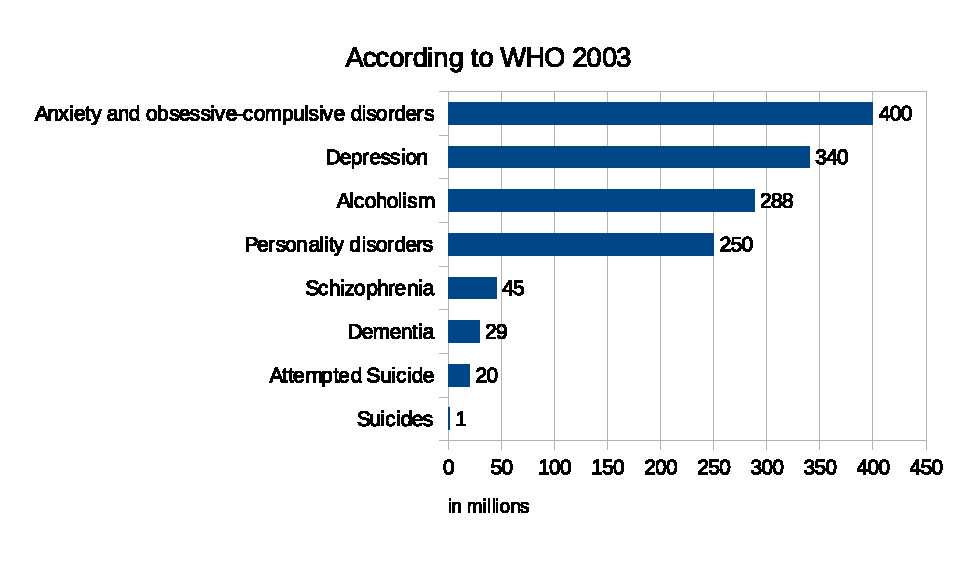
\includegraphics[width=13cm]{Prevalence_Disorders.eps}
\caption{Epistemology of mental disorders (according to an estimate of the WHO 2003)}
\end{figure}

According to a study done by the WHO is world wide every fourth visitor to a doctor affected by mental disorders.
Let's take Switzerland as an example as an affluent country\footnote{Yet another reason is, that this 
	original material which has been translated originates from Switzerland.}.
	% Numbers from the USA
In Switzerland, 25\% -- 40\% of the patients of family doctor's offices suffer partially or exclusively from mental disorders. The biggest part of these cases go undiagnosed and untreated.

According to the Swiss Health Observatory, mental disorders are significantly above average in intentional comparison. Roughly half of the people living in Switzerland suffer at one point in their life from a mental disorder. Depression and anxiety make a big part of it.

The majority of the Swiss consider themselves healthy and mentally stable. Nevertheless are about 25\% of the population affected by a mental disorder, which allow a diagnosis.
But just 5\% seek psychiatric or psycho--therapeutical help. 

So in Switzerland in the year 2000, out of 7.2 million, 146,000 people were treated by psychotherapists. But it is assumed that there would be a need for about 553,000 people. Even if we assume that not all of these mental disorders have to be treated by a doctor, we can nevertheless see a significant under--supply in this domain. But it's safe to assume that some of these people might seek help outside the established health care system, so for instance also with stress regulation trainer.

Now these numbers were for Switzerland which in many points stands out as a safe, affluent and welcoming country. So when the situation was that bad in a very well off country, that shows how much this situation might be lacking elsewhere, where there are not the same means.
%Check which year written, adapt this number and say which year 

\epigraph{It isn't obvious at all, the the sick person wants to get healthy. Something in the sick person is in secret complot with his disease.}{translated by author from \textit{Wilhelm St\"ahlin}}


1\% of the Swiss population goes to stationary treatment, and a fifth of them not on their own accord.

\begin{table}[htb]
	\centering
\begin{tabular}{ll}
	Men: & Women: \\
	\hline
	Drug abuse & Heavy Depression \\
	Alcohol abuse & Alcohol abuse \\
	Schizophrenia & Schizophrenia \\
	Heavy Depression & Neurotic disorders \\
\end{tabular}
\caption{The four most common diagnoses for a hospitalization in Switzerland.}
\end{table}

So that means that in a space of 12 months in Switzerland:
\begin{itemize}
	\item about 10\% of the Swiss population (600,000-800,000) suffers from a serious mental disorder.
	\item 1\% (60,000-80,000) fall ill every year.
\end{itemize}

Especially the age groups of the young adults (18--25 years) and the elderly people (above 74 years old) were especially affected by that under--supply. 
It is common in these groups, that people don't indicate psychological disorders, but nevertheless suffer from them (particularly pronounced in men). This under--supply is worse in rural areas than in cities.
Insufficient supply means for a person a heightened risk for the severity to increase and/or the disease becoming chronic\footnote{The disease slowly develops and becomes permanent.}. 
In the worst cases, this can lead to suicide.
Out of that reason, early recognition of these conditions is very important.
In order to reach this goal, it is paramount that specialists like stress regulation trainers, but also the general population to be better informed as the chances to be confronted by it are high.

For young people, suicide is the second most common cause of death. In Switzerland, more people die by suicide than traffic accidents, AIDS and drugs combined. 
That puts this first world country high up in the world wide statistics.
Men commit suicide twice as likely as women. 
2002, in Switzerland 979 men and 465 women commit suicide.
Contrary to that, women much more often \emph{attempt to commit suicide}.
According to estimates, between 8,000 and 15,000 people in Switzerland attempt to commit suicide every year.
According to one study of 2002, 8\% of the 12--16 year old girls and 3\% of the girls have already attempted to commit suicide.
Only a small part of these teenagers received therapeutic support afterwards.
Studies show that about 2\% of the Swiss population went through a serious attempt to end their lives (compare to section~\ref{sec:suicide} on page~\pageref{sec:suicide}). 
\end{document}

